\chapter{Практическая часть}

\section{Задание \No{}1}
Представления списков, указанных в условии данной лабораторной работы, в виде списочных ячеек изображены на рисунках 0.1-0.6.

\begin{enumerate}
    \item '(open close halph)
        \begin{figure}[H]
            \centering
            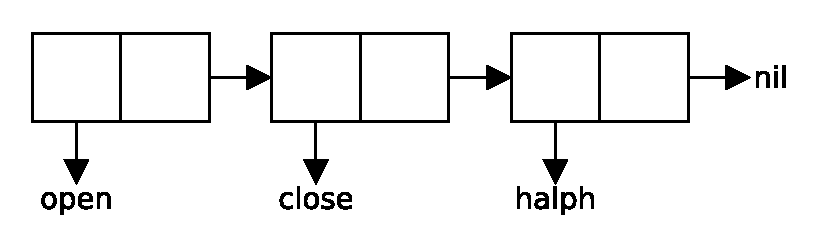
\includegraphics[scale=0.75]{data/pdf/01-01.pdf}
            \caption{Список '(open close halph)}
        \end{figure}
    \item '((TOOL) (call))
        \begin{figure}[H]
            \centering
            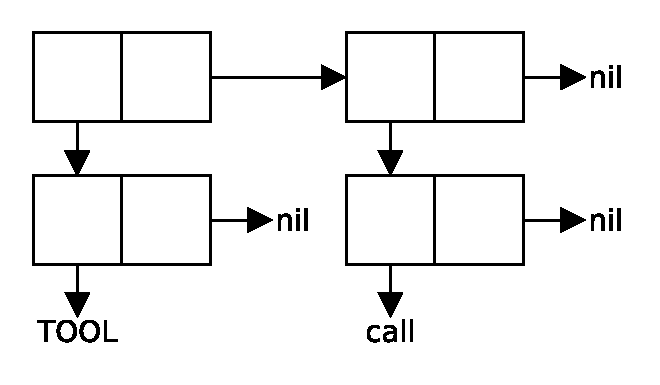
\includegraphics[scale=0.75]{data/pdf/01-02.pdf}
            \caption{Список '((TOOL) (call))}
        \end{figure}
    \item '((open1) (close2) (halph3))
        \begin{figure}[H]
            \centering
            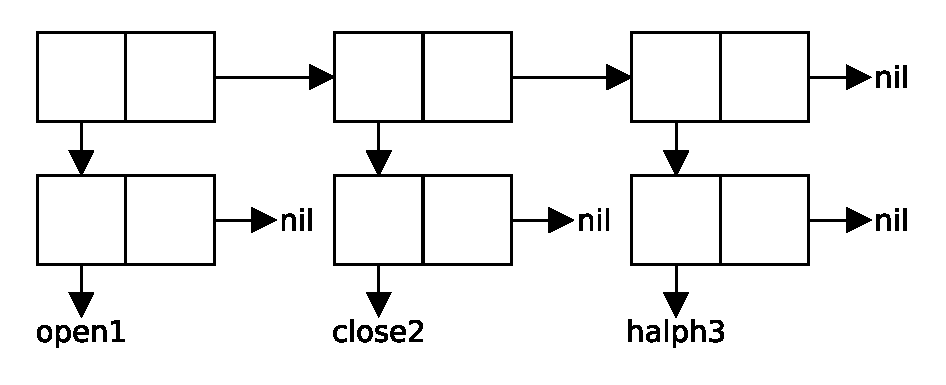
\includegraphics[scale=0.75]{data/pdf/01-03.pdf}
            \caption{Список '((open1) (close2) (halph3))}
        \end{figure}
    \item '((TOOL1) ((call2)) ((sell)))
        \begin{figure}[H]
            \centering
            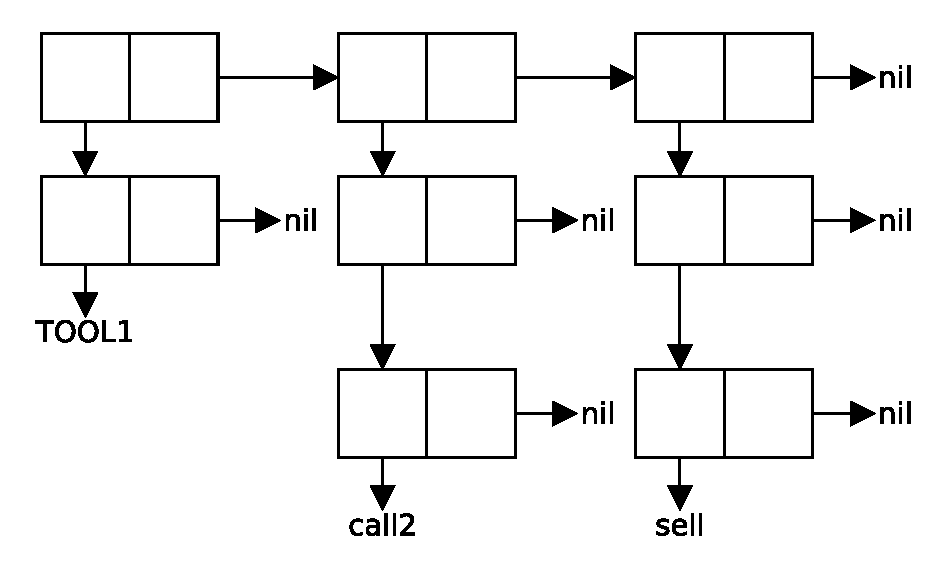
\includegraphics[scale=0.75]{data/pdf/01-04.pdf}
            \caption{Список '((TOOL1) ((call2)) ((sell)))}
        \end{figure}
    \item '(((TOOL) (call)) ((sell)))
        \begin{figure}[H]
            \centering
            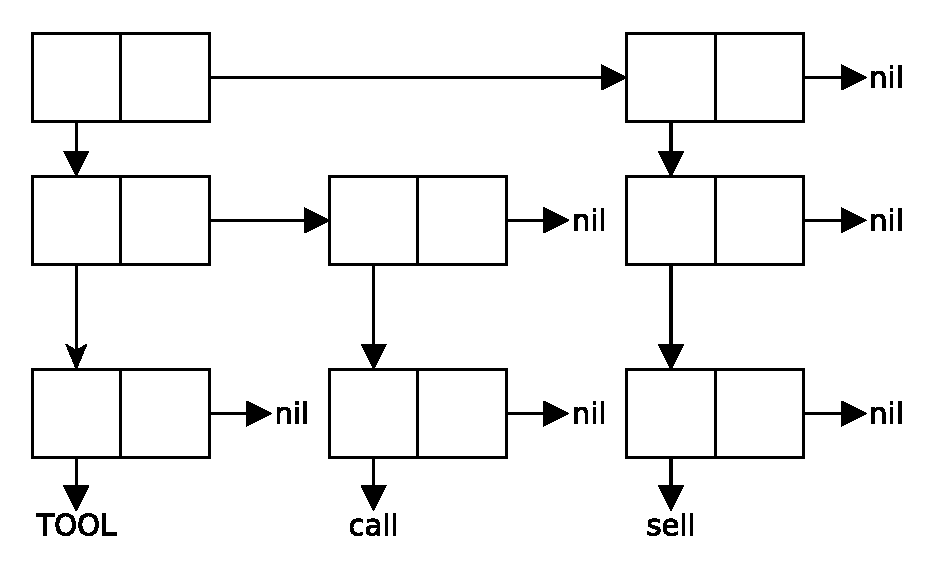
\includegraphics[scale=0.75]{data/pdf/01-05.pdf}
            \caption{Список '(((TOOL) (call)) ((sell)))}
        \end{figure}
    \item '((one) for all (and (me (for you))))
        \begin{figure}[H]
            \centering
            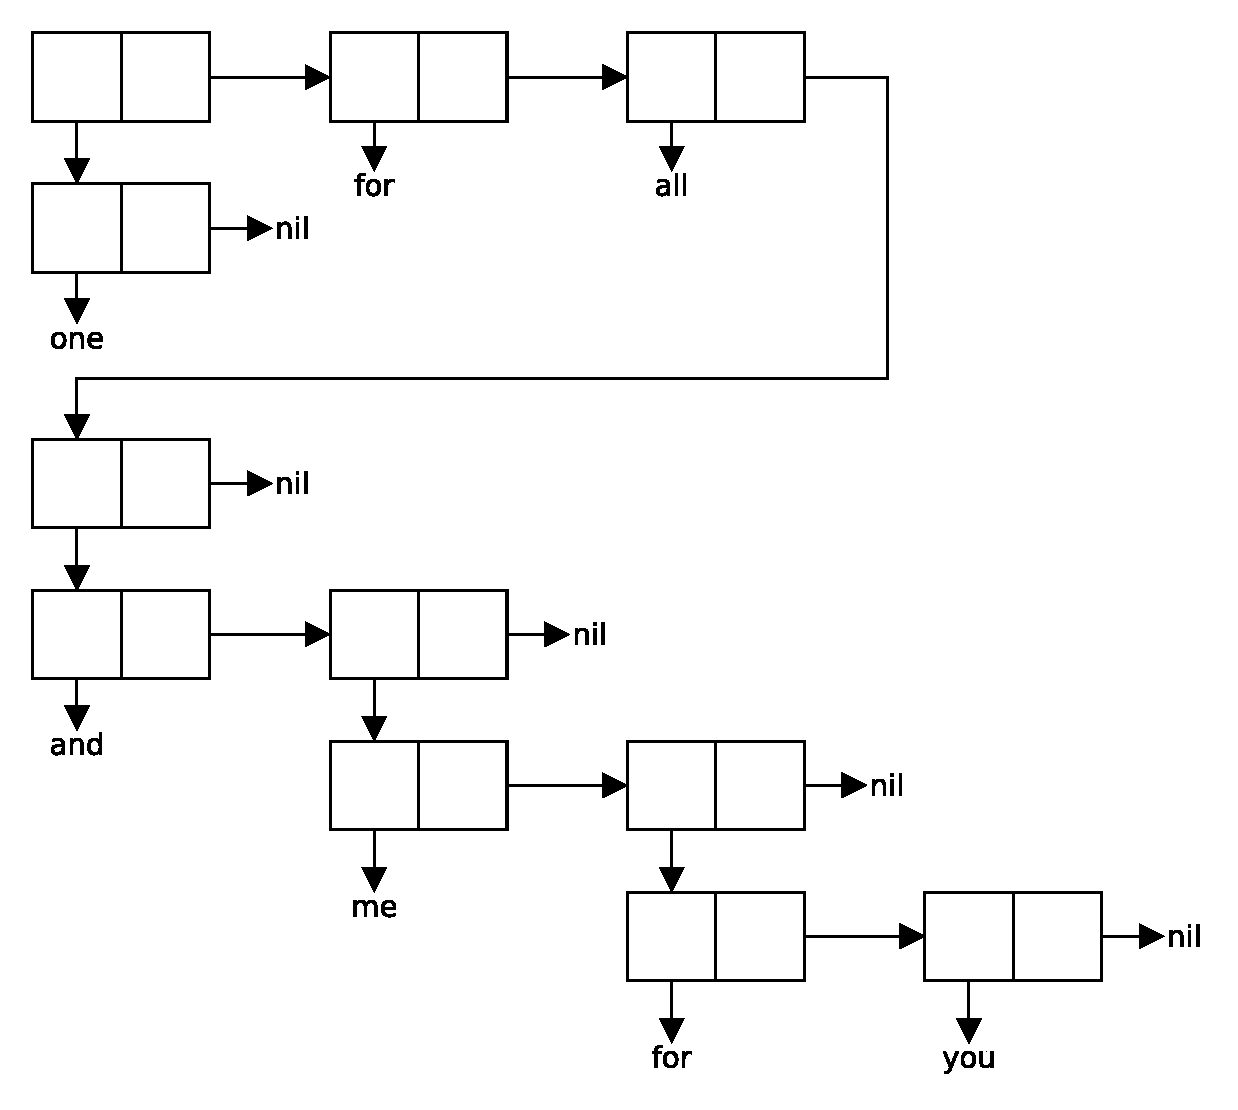
\includegraphics[scale=0.75]{data/pdf/01-06.pdf}
            \caption{Список '((one) for all (and (me (for you))))}
        \end{figure}
\end{enumerate}

\section{Задание \No{}2}

В листинге 1 приведены три выражения на языке Lisp, которые возвращают второй, третий и четвёртый элемент списка '(1 2 3 4 5) соответственно.

\lstset{language=lisp}
\begin{lstlisting}[caption={Выражения, возвращающие 2, 3 и 4 элементы списка}]
(car (cdr '(1 2 3 4 5)))
(car (cdr (cdr '(1 2 3 4 5))))
(car (cdr (cdr (cdr '(1 2 3 4 5)))))
\end{lstlisting}

